\section{Data Interpretation}
\label{section: tracking method - data interpretation}

\begin{figure}[h]

    \begin{subfigure}{0.5\textwidth}
        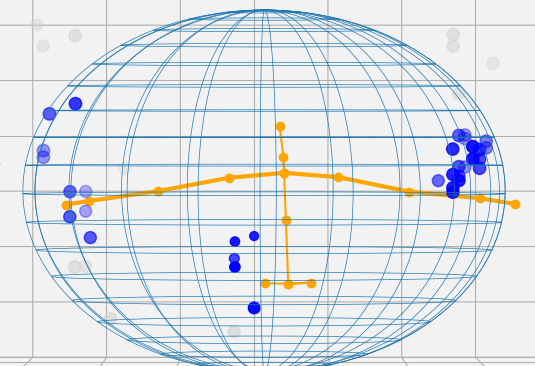
\includegraphics[width=0.9\linewidth]{figures/internal data/IAmMuse internal view.png}
        \caption{Internal data view}
        \label{figure: internal data view, a}
    \end{subfigure}
    \begin{subfigure}{0.5\textwidth}
        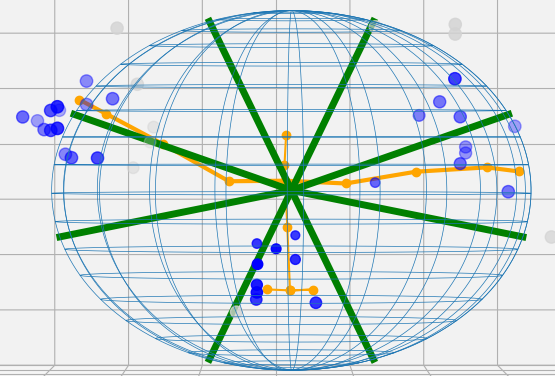
\includegraphics[width=0.9\linewidth]{figures/internal data/IAmMuse internal view with zones.png}
        \caption{Internal data view with zones}
        \label{figure: internal data view, b}
    \end{subfigure}
    
    \caption{Internal data view}
    \label{figure: internal data view}
\end{figure}
% \textbf{¡¡¡¡ The explanation is quite difficult to follow currently, think up specific terms and meanings, in order to make the explanation more clear!!!}\\
% Things to get a specific term for
% \begin{itemize}
    % \item MEB center
    % \item MEB radius
    % \item MEB circle (for reasoning)
    % \item specific arm zones, e.g. left low; left mid; left high; right low...
    % \item angle ranges
% \end{itemize}

The method used for data interpretation is tightly linked to the method used for data enhancement, since the data enhancement method adds a specific type of information to our input data.
In the case of IAmMuse, we have the ball, which encompasses the user, as well as the extra dimension of weight, added to the point cloud.
The data interpretation method of IAmMuse will thus be built around this new information.
A visualization of this internal state, with the ground truth in orange, is shown in \cref{figure: internal data view}.


\subsection{Conceptually}
\label{sub-section: tracking method - data interpretation - conceptually}

% What do we want to predict
As was mentioned at the start of \cref{chapter: tracking method}, the goal of IAmMuse is to predict what \textit{zone} a specific hand is in.
These zones are defined as being a \textit{range of angles}, and can be either "low", "middle", or "high". 
Respectively representing situations where the user points at the floor, outwards, or at the sky.
% 2D simplification.
When reasoning about this system, a useful simplification is to think about the system in two dimensions.
This would change our enclosing ball into a circle, enclosing the movement space of the user's arm, where the center of the circle is still at the user's sternum, and the edge still traces the potential positions of the user's hands. 
Each 3D point would then be transformed into its 2D projection, where we remove the direction outwards from the mmWave camera.
The reasoning performed on this simplified model still holds in the actual model, why this is the case will be specified throughout \cref{sub-section: tracking method - data interpretation - practically}.


% pointcloud -> angleset
Since each point can be interpreted as a prediction/reading of the position of the arm, it's also possible to determine a prediction/reading of the angle of the arm, as predicted by that singular point.
This \textit{point angle} can be defined as the angle of the line which goes from the user's sternum (center of the enclosing circle) to that specific point.
This allows us to transform our weighted pointcloud into a set of predicted angles, with a weight equal to the original point weight, which represents the "value" of that particular prediction.
With this list of weighted angles, it's now easy to make some likelihood predictions for specific arm zones by simply looking at the zone in which each angle falls and the weight of that angle.


\subsection{Practically}
\label{sub-section: tracking method - data interpretation - practically}

% Pointcloud -> angleset
The first step that needs to be performed is to transform the weighted point cloud into a set of weighted angles, corresponding to the angle which the arm would have if it went through the specific point.
To calculate this angle, the vector between the center of the enclosing ball and the specific point considered is taken.
Then the arc-tangent of this vector's distance in the X-axis (side to side) and the Z-axis (up-down) is considered to be the angle of the point.
Since the user is expected to hold their arms out mostly straight, the user can be correctly assumed to be roughly two-dimensional.
From this, we can see that the encompassing ball can be viewed as an encompassing circle, since the center of the circle is said to be at the location of the user's sternum, and is thus at the same distance from the mmWave camera as the user.
% \textbf{INCLUDE THIS?}
A better method would have been to consider the angle between the aforementioned vector and the down vector, making a distinction between "left" and "right" based on the sign of the X component of the vector.
This would allow the user to hold their arms somewhat more forward without affecting the accuracy of the system.
In this case, the simplified two-dimensional reasoning still applies, as you can take an X-value in the 2D space as being $\sqrt{x^2 + y^2} \times \text{sign}(x)$.
% \textbf{END OF INCLUDE THIS?}
Doing this for all points in the weighted point cloud yields us a list of angles with an associated weight.

% angleset -> prediction
Each arm zone is internally defined as a range of angles, where a zone should thus be selected if the specific arm is within that specified angle zone.
The way IAmMuse differentiates between the left hand and the right hand is simply by the angle.
These angles exist on a range between $0\degree$ and $360\degree$, where $0\degree$ is down, $90\degree$ is left, $180\degree$ is up, and $270\degree$ is right. 
In this way, systems can be generalized over both arms.
Each arm zone then gets a weight equal to the cumulative weight of all the angles that fall within its angle range, only considering angles from one frame.
The right and left zones with the highest weight are then predicted to be the zone where the user's hands are currently.
Making sure only to select \textit{one} left zone and \textit{one} right zone.

% Why we need stabilization
% This system has a few issues, though. 
% For one, very sparse frames currently have the same effect as very dense frames, while the information present in a sparse frame is, by definition, lower.
% Since the mmWave radar has frames where it simply produces less, and less useful data, it often happens that a small bit of noise will produce an almost random prediction on these frames.
% Even on denser frames, it's possible for large noise spikes to poison a specific prediction.
% Lastly, there is the issue where an arm located at the edge of two zones will be predicted to be one or the other almost at random for any particular frame, due to the inherently random point distribution point samples generated by the mmWave radar.
% While this is not a big deal when it comes to a single frame, during system usage, this means that the system might rapidly change its prediction back and forth, resulting in a non-stable output on a stable input (user arm position), which is a bad thing.
% For these reasons, it's important to consider methods for data stabilization.

\subsection{Data Stabilization}
\label{sub-section: tracking method - data interpretation - data stabilization}

% stabilization intro & minimal points
There are a few issues with the current system, though, all to do with the stability of the resulting prediction, and extra systems have been put in place to mitigate these issues
Firstly, one issue occurred when the mmWave radar produced very sparse frames. 
Sparse frames contain disproportionately few points, and thus also contain disproportionately few signal points. 
This means that the predictions of IAmMuse are more susceptible to the random variations in the point distributions, as well as being more susceptible to noise, since the prediction system simply looks at which zone has the highest weight.
The way in which IAmMuse mitigates this issue is by setting a \textit{minimal weight} which a zone must have to be considered as a "valid prediction", if no valid prediction was made for a side, the previous prediction is kept.
This mitigation strategy does have the side effect of ignoring some frames if they are too sparse, but this isn't a huge problem, as the amount of information present in that frame was already very low, by way of how sparse it was.
A solution that adds the data from these "missed frames" to the following frames could be made.
This would increase the amount of information the system uses, but could also induce a lower responsiveness by taking into account stale information.
For these reasons, such a system was not put in place in IAmMuse.


% Multiple predictions needed
Another similar issue occurs when a large spike of noise is perceived for a single frame, this influx of faulty data can make the system select an incorrect zone.
These large noise spikes do not happen regularly, but they happen often enough that a mitigation system was useful.
In these cases, most frames in a sequence will give a similar result, but one frame will give a "faulty prediction".
Since we know that, in a correct set of frames, the same zone would likely be predicted multiple times in a row, as the user's arm stays in that zone, we can filter out the faulty case by only choosing a new zone if that zone has been predicted twice in a row.
In this system, it's important not to count "missing predictions" (as specified in the previous paragraph) as a part of these consecutive predictions.
This system does add some delay to the selection of a new zone, specifically 100ms if you receive correct predictions every frame. 
For the IAmMuse system, this delay is a worthwhile tradeoff for the added stability against both noise and random fluctuations in the mmWave radars' output, but this may not be the case for every system.

% Zone expansion
Lastly, IAmMuse had to solve an issue in the scenario where a user is holding their arm near the border of two zones.
In this case, IAmMuse may predict either zone at random, purely due to the random nature in which the points in a mmWave frame are distributed.
While a singular frame prediction would not be incorrect per se, the fact that the system produces an unstable output while the user provides a stable input (a stationary arm) is incorrect.
The way that IAmMuse solves this issue is by expanding the region assigned to the currently selected zone.
This eliminates the issue, as the randomly distributed points that are on the edge of the two zones will be predominantly in the active zone if the zone's angle range is increased.
In IAmMuse, the active zone's angle range is increased by $10\degree$, or $5\degree$ on each side, and neighboring zones are shrunk in accordance.
This increase should be as small as possible while still providing the stability-increasing effect.
During system design, an increase of $10\degree$ seemed to be the smallest amount that fulfilled this wish.





% The data interpretation method is often tightly linked to the data enhancement method used, as we will use the extra context provided by the data enhancement in the interpretation.
% In the case of IAmMuse's final system, the extra context we've been given is the MEB, providing us with a rough center point of the user, as well as an estimation of the outer reach of their arms.
% % simplify to 2d explained
% During the design and explanation of the interpretation algorithm, we will often simplify the user's points to be on a plane, rather than in 3d space. 
% The MEB would then likewise be considered to be a circle, with the center still at the user's sternum, and the edge tracing the path the user's hands can trace (assuming outstretched arms).
% This estimation makes the reasoning a lot more intuitive. At the end of the section, we will also briefly touch on why this reasoning also extends to our actual system, which does operate in 3d space, rather than 2d space.
% % continue
% The main idea which is used in the interpretation of the data is that the angle of the arm is very closely modeled by looking at the angle between the sternum and a user's hand.
% The sternum position is already known to be roughly at the center of the MEB, and the user's hands are known to be roughly at the edge of the MEB circle.
% This transforms our problem of "find the angle of the arms" to "find the position of the hands on our circle", which turns out to be a lot simpler.
% 
% To find the angle of the arms, a few things need to be done: points that belong to the hand should be specified, these points should be placed on the MEB circle, the angles between these points and the MEB center should be calculated, and this set of angles should be transformed into a hand/arm angle prediction.
% The first step is done in a somewhat different way. 
% We know that the points at the circle edge tell us a lot of things about the position of the hands, and the further away a point is from that circle edge, the less we trust the information. 
% Since your arm position tells you something of where the hand is, but your torso won't tell you anything.
% For this reason, each point is given a \textit{weight}, dependent on its distance to the circle edge.
% In practice, this is achieved by taking the distance between a point and the MEB center, and applying the Gaussian function to this distance, where $\mu$ is the radius of the MEB, $\sigma^2$ is taken to be $0.25$, and x is the previously mentioned distance.
% The output of this function is used as a weight of the point, which is representative of "how hand-like" the point is.
% Calculating the angle for each point is a trivial trigonometric function, and will leave us with a set of angles with weights.
% 
% The last part of the interpretation is turning this list of angels and weights into two final arm positions, one for the right arm and one for the left arm.
% In this thesis, we do not care about the exact arm position, rather, we care about the "region" where the arm currently is.
% This region is specified as being "low", "middle", or "high", which are simply ranges of angles in which the arm can be.
% The fact that the system is expected to generate an output region can be used in the interpretation.
% To find out the likelihood of an arm being present in a specific region, you can look at the "weight" of said region, where a region's weight is the sum of the weights of all points (angles) that exist in that region.
% In this manner, a frame-specific prediction for the arm location can be generated by selecting the zone with the highest weight on each side (left, right).
% One problem with this approach is that the output is very unstable.
% 
% A few methods are used to stabilize the output of the arm location predictions.\\
% Firstly, the arm position (low, mid, high) that is currently selected will increase the angle range that it considers "its region" by $5\degree$ on each side. 
% e.g. the middle zone usually considers points "in its zone" when their angle is between $65\degree$ and $105\degree$, but if the middle zone is already selected, it will now consider angles between $60\degree$ and $110\degree$, this region increase will shrink the other regions.
% This system avoids the situations where a user's arm is "on the edge" of two zones and rapidly changes which zone is predicted while the user keeps their arm still.\\
% Secondly, there is a certain threshold weight that a zone needs to achieve to be considered as a "valid zone contender", this makes sure that very sparse frames can not trigger a faulty zone change based on only a few points.\\
% Lastly, a specific zone is only selected as the actual zone if it was predicted to be the correct zone twice in a row.
% Note that some frames may not have any predictions at all if none of the zones crossed the weight threshold, in this case, no prediction was made, thus it does not impede a zone from being chosen twice.
% e.g. \textit{frame n}, zone left low is selected. \textit{frame n+1} no zone is selected. \textit{frame n + 2} zone left low is selected.
% In this situation, \textit{left low} has been selected twice in a row, thus, the zone gets set to left low.
% 
% Earlier in the section, it was stated that we could reason about the minimal enclosing ball as if it were a circle, the reasons for this assumption will be given here.
% First off, during the usage of the system, the user is expected to stand facing the FMCW, with their arms out to the side, lifting or lowering them.
% In this situation, the point cloud produced by the user falls roughly in a plane where we simply ignore the y direction, thus, for the points belonging to the user, the simplification to a circle is valid.
% Furthermore, the number of noise points that still exist in this part of the pipeline is small, and given the spatial distribution observed from these points, the likelihood of one of these points being present near the edge of the ball but in front of or behind the user is very slim.
% Therefore, only outlier points will ever appear near the edge of the ball while not being well modeled by the circle.
% Points that are at a large distance from the edge of the ball will be disregarded automatically by being assigned a low weight, as the distance between the centroid and the specific point can be (and is) calculated in 3d.
% Due to the above given reasons, there is no feasible situation in which the assumption (for reasoning purposes) of a circle does not apply accurately to our actual ball.
% Lastly, it's important to mention how we get the "angle" between two points now, given that we are not actually using 2d coordinates in the system.
% The angle of the arm is considered to be the angle between the down vector and the vector that goes from the MEB circle to the point in question.
% This has the added benefit that users are allowed to hold their arms at a somewhat forward angle if this is more comfortable for them, and the calculation still holds true in the same manner.



% % This section describes HOW we do the data interpretation, given the different systems described above, specifically the minimal enclosing ball.
% % This includes the general high-level overview of the system, including zones on the MEB, filtering, and processing.
% % It will also discuss different smaller systems, such as the active zone size increasing code, the stabilization code, which requires a zone to be selected more often, and will discuss the concept of "weight" in the various system contexts.
% % 
% % \textbf{We use a ball, not a circle, explain}